\chapter{Vertices and Transforms}

\section{WebGL at 10,000 feet}
\summary{High-level overview of the WebGL rendering pipeline.}

See Figure~\ref{fig:AssemblyLine}.

\begin{figure}[htb]\centering
  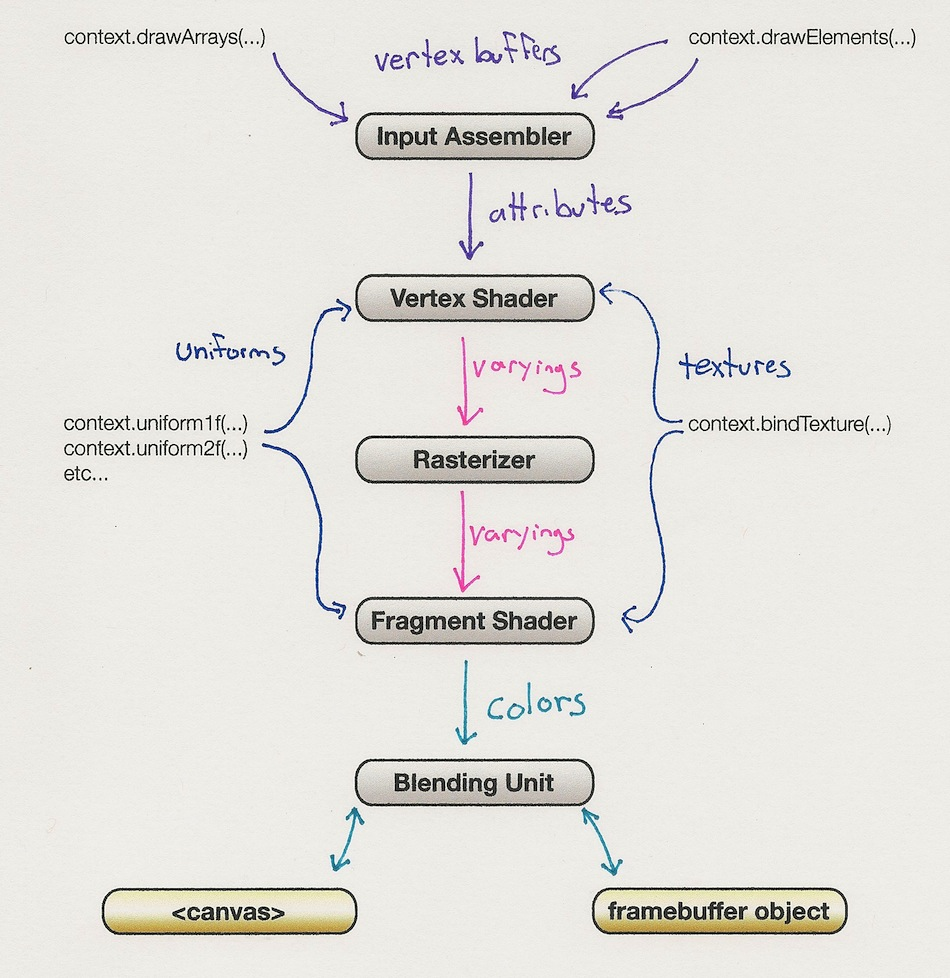
\includegraphics[width=70mm]{pipeline.jpg}
  \caption{High level view of the WebGL / OpenGL ES pipeline}
  \label{fig:AssemblyLine}
\end{figure}

\section{Vector Algebra with JavaScript}
\summary{This sections walks through giza's implementation of vector and matrix classes.  Rotation, translation, and scale are given a very brief treatment.}

\section{Life of a Vertex}
\summary{Describes model, view, and projection transforms.}

\section{Shading Language Basics}
\summary{Explains uniforms, attributes, and varyings.  Walks through trivial \texttt{main} functions for vertex and fragment shaders.}

\subsection{GIZA.FX}
\summary{Describes a useful abstraction of the WebGL program object.}

\section{Lines and Triangles}
\summary{Explains the various primitive types (e.g., \texttt{LINES}), \texttt{drawArrays}, and \texttt{drawElements}.}

\section{Typed Arrays, Vertex Attributes and VBOs}
\summary{Shows how heterogeneous data (e.g., colors and positions) can be interleaved and submitted to WebGL.}

\rrecipe{Recipe 2: Color Wheel}
\summary{Spinning wheel with various colors at each vertex.}

%\rrecipe{Recipe 2: Color Graph}
%\summary{Animated wireframe graph of the sinc function; illustrates performance differences between JavaScript-side computation and shader-side computation.}
